\chapter{Environment}
\label{chapter:environment}

This section will describe the environment used for both the training and testing of the experiments, namely:

\begin{itemize}
    \item In \autoref{section:data} an overview of the dataset along with the necessary steps before training (preprocessing, data split and augmentation) will be presented.
    \item The software stack used for training and testing models will be presented in \autoref{section:software}.
    \item Finally, an overview of the hardware resources used for the experiments will be provided in \autoref{section:hardware}.
\end{itemize}



\section{Data}
\label{section:data}
    The \ac{ISIC} 2019 challenge \cite{isic2019} provides a training dataset with 25331 samples distributed across 8 different categories. Such categories are: melanoma, melanocytic nevus, basal cell carcinoma, actinic keratosis, dermatofibroma, vascular lesion, squamous cell carcinoma and finally benign keratosis (a category which includes samples of solar lentigo, seborrheic keratosis and lichen planus-like keratosis). This dataset is composed by samples of HAM10000, BCN 20000 and MSK, all of which are labelled datasets of skin lesions.
    
    The \ac{HAM10000} \cite{ham10000} dataset is an effort to boost research on automated diagnosis of dermatoscopic images that focuses on the quality and reliability of a large volume of data. All of the samples are manually reviewed by dermatology professionals and non-dermatoscopic images or unreliable diagnoses are filtered out. Finally, all of the samples have the same resolution of 600x450 pixels centered around the lesion. The quality and volume of the data provided by this dataset is remarkably good and allows deep learning researchers to focus on developing reliable models rather than focus on extensive pre-procecssing methods before training. \par
    
    The \ac{HAM10000} had already been used in the task 3 of the ISIC 2018 challenge. The literature suggests that the top scoring approaches of the ISIC 2018 surpassed expert dermatologists \cite{?}, however, as Tschandl et al. pointed out, the algorithms performed worse on images from other dermascopic data sources which were not present on the \ac{HAM10000} dataset. This statement shows that the \ac{HAM10000} dataset alone does not provide enough samples that are representative of real world scenarios, which might be composed of lesion with different pingmentations and the images might be taken under different conditions (e.g. angle, luminosity or contrast variations). \par
    
    As a contermeasure, the ISIC committee added two more datasets to the ISIC 2019 challenge, which would hopefully create enough variation and help ISIC challenge metrics be representative of real world scenarios. One of the new datasets is the BCN20000 \cite{bcn_20000}, which contains hard to diagnose images of size 1024x1014 captured between 2010 and 2016 by the Hospital Clinic in Barcelona. These images are often not correctly segmented, located in hard to diagnose locations such as nails or mucosa, and can even be hypopigmented, meaning  that the overall color of the lesion is lighter than the skin tone. The resulting database includes 19424 manually revised dermoscopic images corresponding to 5583 skin lesions. \par
    
    Finally, the other new dataset is the MSK \cite{msk} dataset,  which contains images of multiple resolutions and multiple aspect ratios. The MSK is composed by multiple datasets, namely:
    \begin{itemize}
        \item MSK-1 which contains Both benign and malignant melanocytic lesions. Almost all diagnoses were confirmed by histopathology reports; the remainder consists of benign lesions confirmed by clinical follow-up. Images were not taken with modern digital cameras.
        \item MSK-2 composed of Biopsy-confirmed melanocytic and non-melanocytic skin lesions. This dataset includes over 500 melanomas. Many images have polarized and contact variants.
        \item MSK-3 containing Assorted images and lesions, mostly nevi and basal cell carcinomas. These images were found based on a search not filtered for any particular pathology. All diagnoses confirmed by histopathology.
        \item MSK-4 having images found based on a search for patients with a personal history, clinical diagnosis, or differential diagnosis of melanoma. All diagnoses confirmed by histopathology.
        \item MSK-5 composed of seborrheic keratoses obtained from patients during a clinical visit. These lesions were not biopsied and were determined to be seborrheic keratoses by agreement of three experts.
    \end{itemize}
    
    By looking at random samples from each of the eight classes of ISIC 2019 dataset from Figure \ref{fig:samples}, one can see that samples are quite different from each other, as they often vary on aspect ratios, luminosity conditions, segmentation, cropping schemes and even the position of the lesion itself. Even within a particular category, a uninstructed person has a hard time to point out common features between the lesions. Overall, due to the heterogeneity of the ISIC 2019 dataset, it likely represents a set of samples more characteristic of real world scenarios as seen by a dermatology professional \cite{?}.  \par
    
    \begin{figure}
      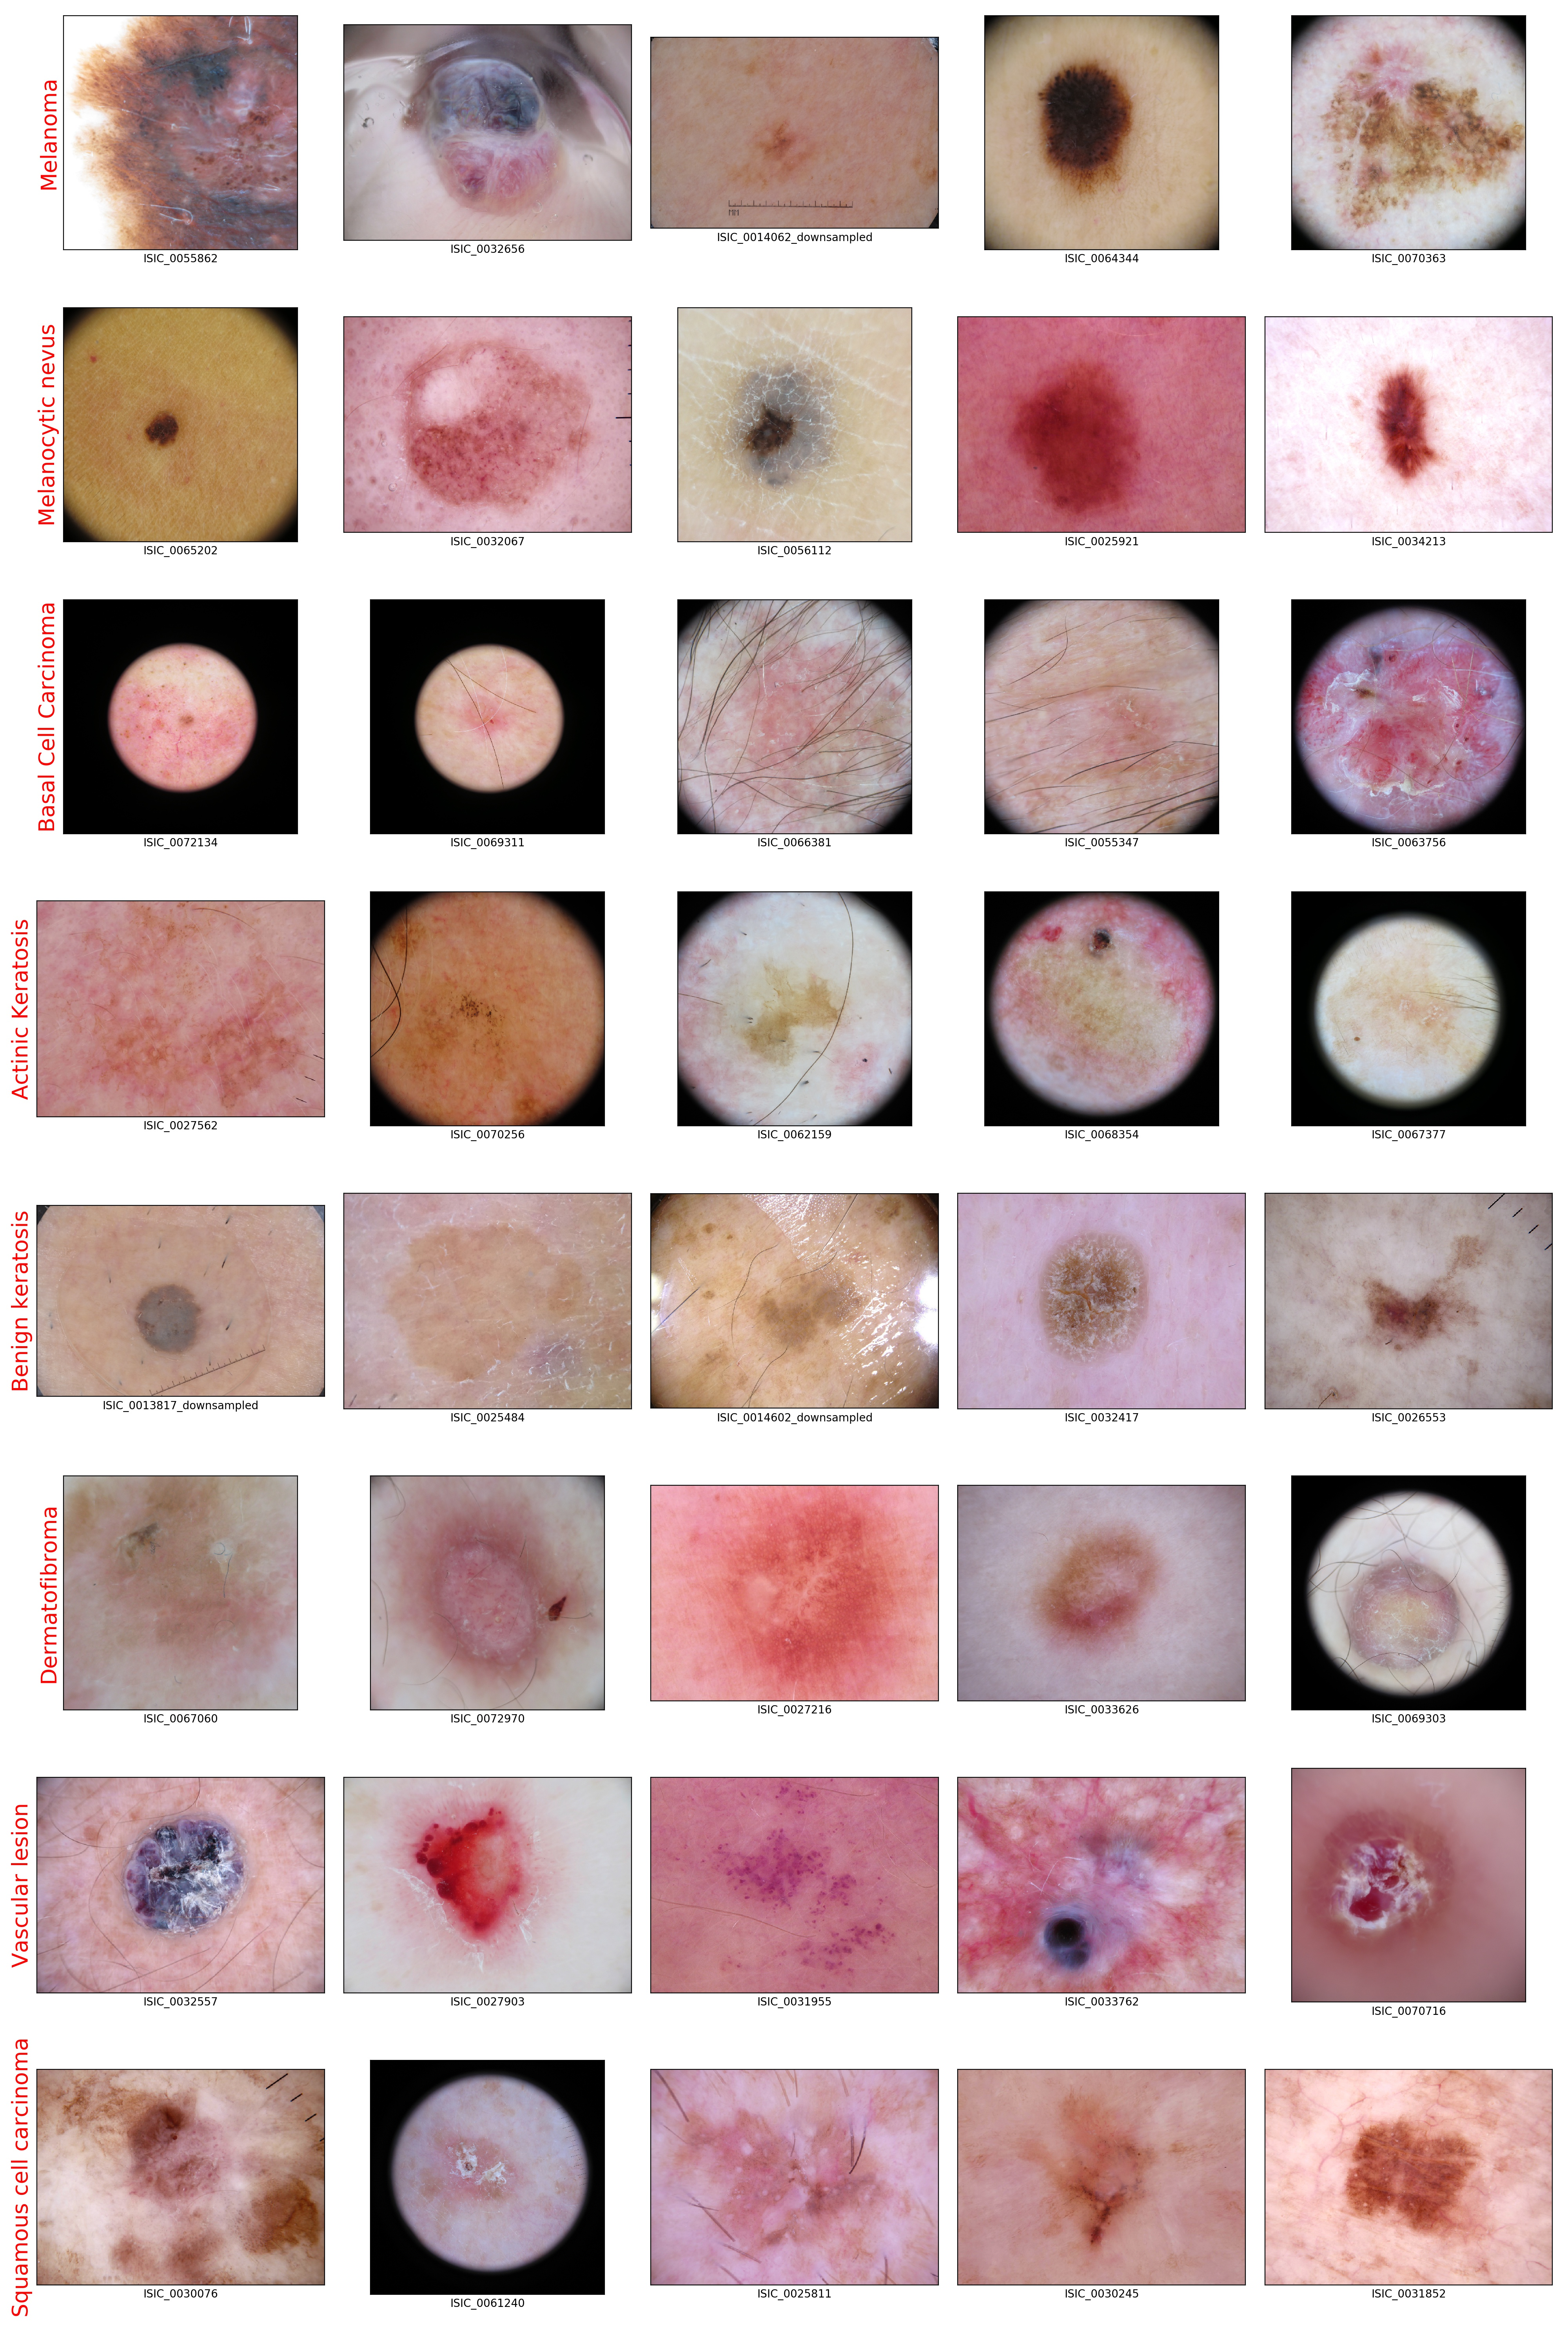
\includegraphics[width=\textwidth]{figs/samples_training_data.jpg}
      \caption{Samples from ISIC 2019 training data for the 8 known categories}
      \label{fig:samples}
    \end{figure}
    
\subsection{Class imbalance}
\label{subsection:imbalance}

    Note that the dataset provided is highly unbalanced with some classes like the melanocytic nevus representing almost half of the whole dataset, while a class like Dermafibroma representing less than 1\% of the dataset On chapter ???? we will present study the effects of this class unbalance and present some strategies to deal with it. \par
    
    \begin{figure}[h!]
      \includegraphics[width=\textwidth,keepaspectratio]{figs/training_data_distribution.jpg}
      \caption{Class distribution of ISIC 2019 training dataset}
      \label{fig:distribution}
    \end{figure}

    To tackle this issue, a common method from the literature \cite{?} is to use some kind of weighted loss function, like the weighted cross-entropy loss function. The weight $W_i$ of each class $i$ is defined by the equation \ref{eq:class_weights}. \par

    \begin{equation}
        W_i=\frac{N}{C*n_i}
        \label{eq:class_weights}
    \end{equation}
    where $N$ denotes the total number of samples in the training set, $n_i$ is the number of samples for category $i$, and $C$ is the number of categories. \par

    Figure \ref{fig:weight_distribution} illustrates that underrepresented classes like dermatofibroma have a considerably higher weight than classes with more samples like melanocytic nevus. This means that the added loss from a misclassified sample of  dermatofibroma will have a much bigger impact than a misclassified sample of nevi. Therefore, this method will avoid situations where the model tries to optimize weights towards overrepresented classes like nevi, rather than optimizing performance for each class individually. \par

    \begin{figure}[h!]
    \centering
      \includegraphics[width=0.7\textwidth,keepaspectratio]{figs/weight_distribution.pdf}
      \caption{Weights for each class of the weighted cross-entropy loss function for the ISIC 2019 training dataset}
      \label{fig:weight_distribution}
    \end{figure}

\subsection{Unknown Class}
\label{subsection:unknown}
    By looking at the the sample distribution across the different classes on Figure \ref{fig:distribution} one can observe that no data is provided for the 9th category, namely, the "Unknown" category. This category is meant to represent none of the other classes, and the idea behind the introduction of this class is to model a more real world scenario. \par
    
    The range of skin lesion diagnosis extends beyond the 8 classes represented in the ISIC 2019 dataset (see Figure \ref{fig:distribution}). As such, when patients show a specific lesion to their dermatologist to diagnose, the lesion interpretation has to consider which type of lesion it represents, possibly not being part of the 8 categories represented in this dataset or possibly not representing a lesion at all, For example, it might be a scar, a bruise or even normal skin. No data is provided for this class because it does not represent a specific category but rather an agglomerate of any skin fraction that is not any of the other 8 lesion categories. \par 
    
    Different strategies to deal with this unknown class will be experimented with in \autoref{chapter:experiments}. However, for the analysis of the effectiveness of the experimented methods, an agglomerate of multiple samples was created to be categorized as unknown samples. Table \ref{tables:out_dist_dataset} shows the distribution of such samples. \par 
    
    \begin{table}[h]
        \centering
        \begin{tabular}{|l|r|r|}
            \hline
            \textbf{Lesion category}           & \multicolumn{1}{l|}{\textbf{Samples amount}} & \multicolumn{1}{l|}{\textbf{Source dataset}} \\ \hline
            Angiofibroma or fibrous papule     & 1                                            & \multirow{6}{*}{ISIC Archive}                \\ \cline{1-2}
            Scar                               & 1                                            &                                              \\ \cline{1-2}
            Angioma                            & 12                                           &                                              \\ \cline{1-2}
            Atypical melanocytic proliferation & 12                                           &                                              \\ \cline{1-2}
            Lentigo simplex                    & 22                                           &                                              \\ \cline{1-2}
            Lentigo NOS                        & 70                                           &                                              \\ \hline
        \end{tabular}
        \caption{Samples per category of out of distribution samples for the unknown class}
        \label{tables:out_dist_dataset}
    \end{table}
    
    Most of the samples come from the ISIC archive and are left out from the ISIC challenge because they do not belong to any of the 8 classes known classes. More specifically, they are part of the MSK dataset, which means that samples follow the same conditions to the other samples from same dataset, which often makes them quite similar to images from the ISIC 2019 challenge training dataset for an uneducated observer (see Figure \ref{fig:unknown_samples}). As such, these samples will receive the same pre-processing as the samples from the training dataset provided by ISIC. \par
    
    \begin{figure}[h!]
        \centering
        \includegraphics[width=\textwidth]{figs/unknown_image_samples.pdf}
        \caption{Randomly chosen samples from the dataset created for the unknown class}
        \label{fig:unknown_samples}
    \end{figure}


\subsection{Preprocessing}
\label{subsection:preprocessing}
    Each sample of the the dataset undergoes a number of preprocessing steps:
    
    \begin{enumerate}
        \item Most readily available pretrained models are of network architectures whose input tensor is of square dimensions (e.g., $224 \times 224 \times 3$). Since the dataset's images are of distinct non-square dimensions, it is necessary to resize them to a square. However, resizing them all naively to the network's input tensor dimensions without regards to the image's aspect ratio means that the input fed to the network is of varying distinct aspect ratios which does not constitute a good start. Therefore, the first step is to crop an arbitrarily-sized square of the center of the image (as per code snippet \ref{code:crop}) which will likely capture the skin lesion, as most images in the training dataset are centered around the lesion. \par
    
        \begin{listing}[ht]
        \begin{minted}{python}
        def _crop(img):
            width, height = img.size
            if width == height:
                return img
    
            length = min(width, height)
    
            left = (width - length) // 2
            upper = (height - length) // 2
            right = left + length
            lower = upper + length
    
            box = (left, upper, right, lower)
            return img.crop(box)
        \end{minted}
        \caption{Function that crops a given image to a square crop of the center of the original image.}
        \label{code:crop}
        \end{listing}
    
    \item Most input tensors from pre-trained model architectures are $224 \times 224 \times 3$, however, more recent architectures such as EfficientNetB2 or InceptionV3 use bigger images to capture more detail. Therefore, images should be resized to the target networks' input dimensions, as soon as possible in the data pipeline in order to reduce the computational costs of any subsequent operations on the images. Images are resized using nearest-neighbor interpolation, as per code snippet \ref{code:resize}.
    
        \begin{listing}[ht]
        \begin{minted}{python}
        def _resize(img, target_size):
            return img.resize(target_size, PIL.Image.NEAREST)
        \end{minted}
        \caption{Function that resizes a given image to the target dimensions.}
        \label{code:resize}
        \end{listing}
    
    \item Based on Gessert et al. of ISIC 2018 task 3 challenge approach \cite{gessert2018}, each image is normalized by subtracting the channel-wise mean of the entire ISIC 2019 training dataset, and then dividing it by the it's standard deviation (as in code snippet \ref{code:correct}). The channel-wie mean and standard deviation of the ISIC 2019 training dataset was calculated beforehand. \par
    
        \begin{listing}[ht]
        \begin{minted}{python}
def preprocess_input(x):
    """Preprocesses a numpy array encoding a batch of images. Each image is normalized by subtracting the mean and dividing by the standard deviation channel-wise.
    
    # Arguments
        x: a 3D or 4D numpy array consists of RGB values within [0, 255].
    # Returns
        Preprocessed array.
    """
    if not issubclass(x.dtype.type, np.floating):
        x = x.astype(K.floatx(), copy=False)
    
    # Convert pixel values from [0, 255] to [0, 1] 
    x /= 255.
    
    # Mean and standard deviation calculated over the entire ISIC 2019 training dataset
    mean = [0.6236, 0.5198, 0.5038]
    std = [0.2422, 0.2235, 0.2315]
    
    # Zero-center by mean pixel
    np.mean(x, axis=(0, 1))
    np.std(x, axis=(0, 1))
    
    x[..., 0] -= mean[0]
    x[..., 1] -= mean[1]
    x[..., 2] -= mean[2]
    if std is not None:
        x[..., 0] /= std[0]
        x[..., 1] /= std[1]
        x[..., 2] /= std[2]
    return x
        \end{minted}
        \caption{Function that normalizes the sample images over the entire ISIC 2019 dataset}
        \label{code:correct}
        \end{listing}
    \end{enumerate}


\subsection{Augmentation}
\label{subsection:augmentation}
    
    Data augmentation is performed using a different range of techniques which it's impact will be explored in \autoref{chapter:experiments}. As illustrated in Figure \ref{fig:distribution}, samples are highly unbalanced across all 8 known classes. We hypothesise that generating more samples (oversampling) of underrepresented classes through techniques such as data augmentation will significantly improve performance of these classes. \par 
    
    Oversampling is done by combining a different array of techniques each with probability of 0.5 towards a randomly picked sample from a specific class. Therefore, the picked sample which will serve as a basis for augmentation will likely be different each time, depending on the number of samples of the class to be oversampled. Additionally, if a sample is picked more than once, there is a high chance of generating a different sample as the augmentations performed will likely different. \par
    
    By generating a different sample each time augmentation is performed, we minimize the risk of the model being trained with the same samples over and over again, possibly leading to overfitting. \par 
    
    The augmentations used take advantage of the  \verb|Augmentor|\footnote{\url{https://augmentor.readthedocs.io/en/master/}} library, which provides a wide range of data augmentation techniques, with specific implementations for the tf.keras framework. The following are the ones used for our data augmentation study:
    
    \begin{itemize}
        \item Horizontal flip
        \item Vertical flip
        \item 90º rotation
        \item Shears
        \item Randomly increase or decrease contrast
        \item Randomly increase or decrease brightness
        \item Randomly increase or decrease color intensity
        \item Tilts from either top to bottom or bottom to top
        \item Tilts from either left to right or right to left
        \item Skew image towards a random corner of the image
        \item Randomly erase a small section of the image
        \item Distort the original image
    \end{itemize}
    
    These augmentations can either be performed before (offline data augmentation) or during training (online data augmentation) and are applied after taking a central crop of the lesion, in order to augment the lesion itself rather than the surrounding area. Figure \ref{fig:augmentations} illustrates examples of these augmentation techniques. One can see that some techniques have a small effect on the original image, while others can significantly change it. \par
    \begin{figure}[ht]
        \centering
        \includegraphics[width=\textwidth]{figs/augmentations.pdf}
        \caption{Examples of augmentations used on \autoref{chapter:experiments}}
        \label{fig:augmentations}
    \end{figure}
    
    More recent transformations such as Mixup \cite{mixup} were also considered, but one could argument that such techniques do not make sense in skin lesion classification, as they would combine multiple lesions into a single image, which would not represent a real world scenario and possibly could make the network learn from these potentially misrepresenting features which even an expert human diagnosis would have trouble with. \par

\subsection{Split}
\label{subsection:split}
    The number of variables in the future experiments would quickly lead to a combinatorial explosion of configurations, so to minimize the computational cost of the experiments a fixed validation scheme will be used rather than a cross validation scheme. To compensate for this lack of averaging over multiple folds of the data (which gives statistical confidence in the results), a fixed seed is set for every \ac{PRNG} as in code snippet \ref{code:seed}, which in practice means parameters are initialized identically between experiments (providing some level of statistical confidence when making comparisons) and guarantees reproducibility.
    
    \begin{listing}[ht]
    \begin{minted}{python}
    def seed():
        from random import seed
        seed(1)
        import numpy.random
        numpy.random.seed(2)
        from tensorflow import set_random_seed
        set_random_seed(3)
    \end{minted}
    \caption{Seed function that is called on every experiment to ensure reproducibility and similar conditions between experiments.}
    \label{code:seed}
    \end{listing}
    
    The original training and test set from \ac{ISIC} 2019 is available for direct download, but the test set is not labelled as that information is used internally by the organization for reporting performance with a multitude of metrics. As such, samples from the training set will be split into proprietary training, validation and test sets. \par
    
    The train with validation and test sets is done is a 80\%-20\% stratified fashion, which means that 5147 samples from the original set will be part of the test set. Often, other authors from ISIC 2019 use splits with a smaller percentage of the test set, however we want to make sure that our results are not biased towards a specific small test set and as such we chose a bigger one. The test set suffers the same preprocessing steps from the training and validation sets (central crop, resizing and image normalization). \par 
    
    The remaining 80\% will be split again into a 80\%-20\% in a stratified fashion for the train and validation sets, respectively.  However, in contrast with the test set these sets will be augmented through offline data augmentation. We believe that by splitting train and test data after the augmentation is performed, one is creating a high bias in the test data as some samples would be variations of samples from the train/validation sets. As such, the test-train split is done before hand from non-augmented samples, as opposed to the train-validation split which happens right before the training routine. \par

\section{Hardware}
\label{section:hardware}
    The presented training tasks require high computational resources, specially in terms of memory and graphic processing power. As such, it was requested to the the Department of Mechanical Engineering at the University of Aveiro, access to their deep learning research server codenamed Deeplar, that delivers such requirements:
    
    \begin{figure}[ht]
        \centering
        \includegraphics[width=0.4\textwidth]{figs/deeplar.jpg}
        \caption{Deeplar, the computer used for the presented research}
        \label{fig:deeplar}
    \end{figure}
    
    It has four state-of-the-art \ac{GPU}s along with a high performance \ac{CPU} and enough \ac{RAM} for this work:
    
    \begin{itemize}
        \item AMD Ryzen™ Threadripper 2950X;
        \item Four NVIDIA GEFORCE® RTX 2080 Ti;
        \item 128GB DDR4 RAM.
    \end{itemize}

\section{Software}
\label{section:software}

    Deeplar runs on a distribution of Linux called openSUSE Tumbleweed 20191004\footnote{\url{https://software.opensuse.org/distributions/tumbleweed}}. The common way to interact with NVIDIA GPUs for parallel computing is through an API called CUDA. Deeplar in particular uses CUDA version 10.2 \footnote{\url{https://developer.nvidia.com/cuda-zone}}. However, for the task of working with deep neural networks NVIDIA provides a library called cuDNN which allows high level frameworks such as Tensorflow or pyTorch to take advantage of the increased computing power of GPUs. Deeplar uses version 7.6.0 of this library. \footnote{\url{https://developer.nvidia.com/cudnn}}.
    
    For managing the training and testing environment several frameworks are available such as pip, virtualenv or anaconda. The choice for the python environment manager was Miniconda\footnote{\url{https://docs.conda.io/en/latest/miniconda.html}}, due to it's smaller footprint and ease of use compared with the other mentioned frameworks. The difference between Anaconda and Miniconda lies in the lack of pre installed packages in Miniconda's case. 
    All the code was written in Python 3.6\footnote{\url{https://www.python.org/}} and took advantage of the following packages:
    
    \begin{itemize}
        \item TensorFlow\footnote{\url{https://www.tensorflow.org/}} 2.0.0. Used as a backend of the Keras framework, currently integrated within Tensorflow at \verb|tf.keras|. This allows for training and testing various models through an high level API;
        \item NumPy\footnote{\url{https://numpy.org/}} 1.15.4 for various vector and matrix operations
        \item Pandas\footnote{\url{https://pandas.pydata.org/}} 1.0.1 for analysing and manipulating with large amounts of structured data.
        \item Pillow\footnote{\url{https://pillow.readthedocs.io/en/stable/}} 5.4.1 for image handling and transformations because of this work's image preprocessing needs.
        \item scikit-learn\footnote{\url{https://scikit-learn.org/}} 0.20.2 for calculating multiple metrics and to split data into train/validation and testing;
        \item jupyter\footnote{\url{https://jupyter.org/}} 1.0.0 for analysing results and creating graphs in a interactive way.
        \item matplotlib\footnote{\url{https://matplotlib.org/}} for visualizing results through  a multitude of graphs.
    \end{itemize}
    
    The following Github repositories were also used to speed up development: 
    \begin{itemize}
        \item Augmentor\footnote{\url{https://www.tensorflow.org/}} 0.2.8. Used as a image augmentation library that provides a wide range of simple and complex augmentation operations. 
        \item EfficientNet Keras\footnote{\url{https://numpy.org/}} 1.15.4. This is a open source implementation of EfficientNets for the Keras framework. Tesnorflow 2.0.0 does not provide a implementation of EfficientNet, however it is schedules for future releases to be integrated within the tf.keras framework.
    \end{itemize}
    
    
